\chapter{Design}



\section{Klassediagram}

\noindent Et klassediagram er et statisk strukturdiagram, som repræsenterer et systems struktur ved at beskrive systemets klasser, deres tilhørende attributter, metoder samt forhold mellem andre objekter.\\

\noindent Et klassediagram der repræsenterer strukturen på vore spil kan ses på figur \ref{fig:class_diagram}.
Som nævnt tidligere i analyseafsnittet og som det kan ses af klassediagrammet, så har vi primært fem klasser at gøre godt med.
På diagrammet er det muligt at observere at de fleste operationer er public, med et minoritet der er private.
Det er også værd at nævne at vi har ingen beskyttede (protected) operationer.
Hvad angår relationer så har vi et spil, der tilhører et sprog (language), hvilket betyder, at mens spillet kører, er det ikke muligt at have flere sprog indstillet af gangen.
I forhold til terningerne, så kan et spil tilhøre to terninger, hvor så to terninger kun kan tilhøre et spil.
Samme opsætning gælder også for spillerne (Player), hvor så et spil tilhører to spillere, mens to spillere kun kan tilhøre et spil.
Sidst men ikke mindst så kan en pengebeholdning kun tilhøre en spiller, og modsat kan en spillere kun tilhøre én pengebeholdning.\\

\begin{figure}[H]
    \begin{center}
        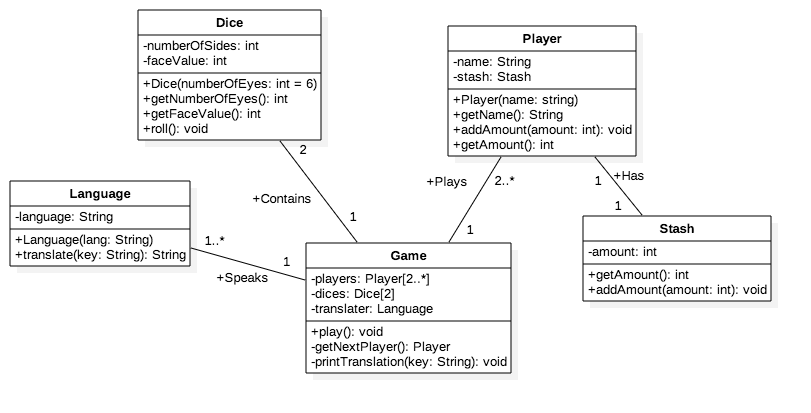
\includegraphics[width=15cm]{graphics/Class_Diagram.png}
        \caption{Klassediagram over spillet}
        \label{fig:class_diagram}
    \end{center}
\end{figure}


\section{Sekvens diagram}

For at illustrere flowet dybdegående har vi lavet et sekvensdiagram.
Dette viser flowet når brugeren begynder at spille.
Det skal dog nævnes, at der på figuren (figur \ref{fig:sequence_diagram}) kun er tegnet interaktionen med en terning, spiller og stash for at holde diagrammet simpelt.
Interaktionen mellem Game og klasser sker dobbelt.

\begin{figure}[H]
    \begin{center}
        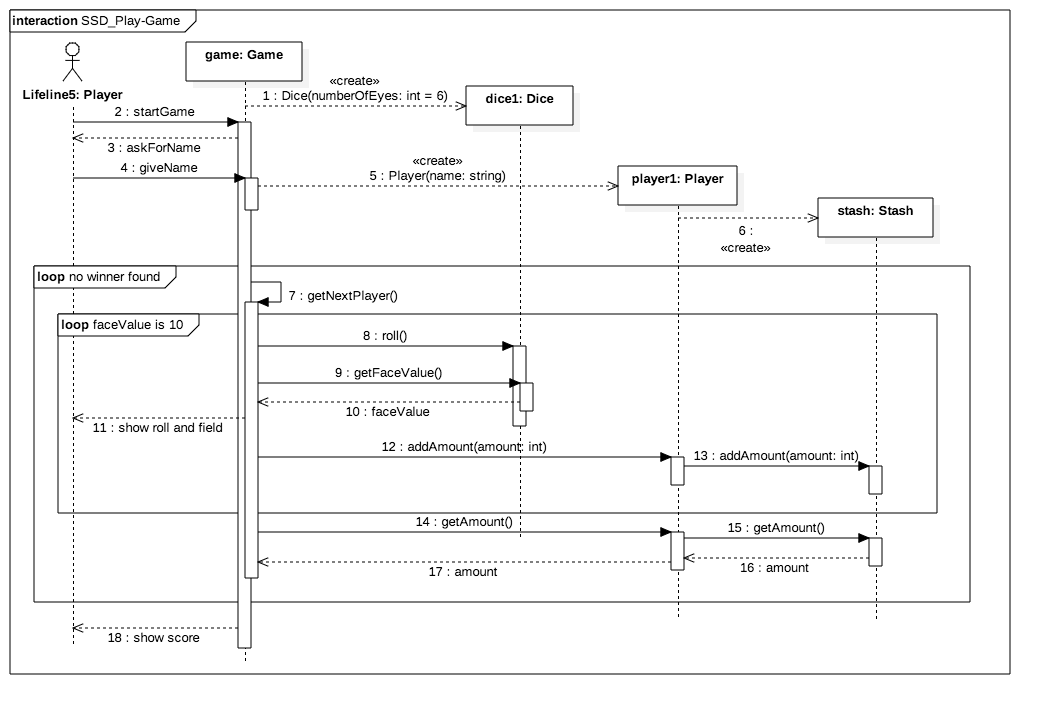
\includegraphics[width=15cm]{graphics/SSD_Play-Game.png}
        \caption{Sekvensdiagram for play game}
        \label{fig:sequence_diagram}
    \end{center}
\end{figure}

\noindent Det ses at når spilleren starter spillet, laver spillet nye terninger og opretter spillerne i systemet, efter den har spurgt efter navne.
Vi kommer nu ind i game-loopet, som vil køre, indtil vinderen er fundet.
Det første der sker her er, at den næste spiller findes.
Terningerne kastes og resultatet for kastet samt feltets oplysninger vises.
Den nuværende spillers pengebeholdning opdateres og loopet starter forfra.
Til sidst vises resultatet.

\newpage

\section{Flowdiagram}

\noindent Et flowdiagram repræsenterer et flow eller et sæt af dynamisk forhold i et system.
Det nedenstående flowdiagram repræsenterer strukuren i hvordan og hvorledes spillet skrider an.\\

\noindent Først og frememst startes spillet, efterfulgt af at der kastes med terningerne og en værdi fastslås.
Efterfølgende beregnes summen af de to værdier fra de to terninger og summen bestemmer et felt.
Dette felt giver på baggrund af værdi en positiv eller negativ indflydelse på pengebeholdning/pointsum.
Er pointsummen større eller lig med 3000, afsluttes spillet.
Er pointsummen mindre end 3000 bliver det den næste spillers tur, hvorefter terningerne kastes igen og den samme process gentages, indtil kriteriet på 3000 i pointsum opfyldes.\\

\begin{tikzpicture}[node distance=2cm]
\node (start) [startstop] {Spillet startes};
\node (kast) [process, below of=start] {Terningerne kastes};
\node (sum) [process, below of=kast] {Summen bestemmer felt};
\node (felt) [process, below of=sum] {Feltet giver point};
\node (hvis) [decision, below of=felt, yshift=-1.5cm] {Pointsum $\geq$ 3000?};
\node (nyspiller) [process, left of=felt, xshift=-4cm] {Næste spillers tur};
\node (vinder) [startstop, below of=hvis, yshift=-1.5cm] {Spillet afsluttes};
\draw [arrow] (start) -- (kast);
\draw [arrow] (kast) -- (sum);
\draw [arrow] (sum) -- (felt);
\draw [arrow] (felt) -- (hvis);
\draw [arrow] (hvis) -- node[anchor=east] {Ja} (vinder);
\draw [arrow] (hvis) -| node[anchor=north] {Nej}  (nyspiller);
\draw [arrow] (nyspiller) |- (kast);
\end{tikzpicture}